
%---------------------------------------------------------------------------------------------------------------------------------------------------------------------------------------------------------------------------
%\newpage
%\setcounter{page}{2}
\renewcommand{\baselinestretch}{1.3}
\onehalfspace

\section{The Model}

This is a perpetual youth economy with heterogeneous agents where the mortality rate is a function of the endogenously determined individual HIV status. There is an exogenous fertility rate that feeds newborns into the economy at a constant rate $\psi$. Agents differ in asset holdings, $a$, in education level, $e$, income shocks $s$, HIV status, $h$, and sex type $i$. The education level is permanent and exogenously given at the beginning of life. The sex type states whether agents are sex consumers or sex producers and is permanent and exogenously determined.\footnote{\sf That is, we focus on endogenezing the intensive margin of sex and leave out from the model the endogenous decision on who becomes a sex consumer or a sex producer. This is clearly a caveat of this exercise which is overcome, for example, by XXX. However, the fact that we introduce a substantial degree of endogenous heterogeneity within each of the two groups implies that part of our sex consumers will consume a positive but negligible amount of sex, and part of our sex producers will produce a negligible amount of sex. The size of this population for which sex transactions are small, which is endogenous, determines the size of the population that consumes/sells risk sex.}

The economy transits across aggregate HIV stages, $g \in \mathcal{G} =\{0,1,2,3\}$, through a sequence of unexpected shocks that reflect the evolution of the HIV epidemic. At stage 0, the economy lives in a stationary pre-HIV epidemic era; at stage 1, the HIV epidemics starts, but agents are unaware of its workings; at stage 2, agents start to learn the sexual nature of the process of HIV infection and the speed of learning differs by education group; finally, at stage 3, ARVs are introduced.


Let us cast the household problem recursively within and across aggregate HIV stages and then explain it. 

\subsection*{[Stage 0] The Pre-HIV Era}\label{sec:stage0}

At this stage, there are not individuals infected with HIV. In this stage, at any given period $t$, agents with asset holdings, $a \in \mathcal{A}$, in education level, $e \in \mathcal{E}$, and income shocks $s \in \mathcal{S}$ solve the following problem depending on their sex type, $i \in \mathcal{I}$: %HIV status, $h=\{-,+\}$, and sex type $i \in \mathcal{I}$.

\noindent \textbf{Risky sex-consumer household problem.} Sex consumers choose consumption $c$, non-marital risky sex $x$, and next period's asset holdings $a'$ to solve the following dynamic problem:
\begin{align}
V(a,e,i,s,\Phi) &= \mathop{\max_{c\geq 0,x \geq 0,a' \geq 0}}  u(c,x) + \beta \gamma \sum_{s'|s}\pi(s'|s)V(a',e,i,s',\Phi') \label{eq:DPi}\\
\mbox{s.t}\nonumber\\
c+ p(\Phi)x +a'&= zy(e)s + (1+r(\Phi))a \label{eq:BCi}\\
s' & = \rho s + \varepsilon \label{eq:varepsilon} \\
a' &\leq \underline{a} \label{eq:borrowing}
\end{align}
 That is, sex consumers derive utility from $c$ and $x$, and discount future at factor $\beta$ times a survival probability $\gamma$. We use consumption as numeraire and the relative price of sex is denoted by $p$. Agents can save and borrow $a'$ in zero net supply with interest rate $r$ and borrowing cannot exceed an exogenous limit $\underline{a}$. Labor income is the product of a permanent component $y(s)$ that depends on the level of education, a transitory component $s$ that follows a Markov process and a permanent component $z$ that depends on individual HIV status and is equal to one for HIV- individuals, We assume that $y(s)>y(\widetilde{s})$ for $s>\widetilde{s}$. 
 
 
 
\noindent \textbf{Risky sex-producer household problem.} Sex-producer households choose consumption $c$, the fraction of time devoted to sex production $l$, and next period's asset holdings $a'$ to solve the following dynamic problem:
\begin{align}
V(a,e,-i,s,\Phi) &= \mathop{\max_{c\geq 0, 1\geq l\geq 0,a' \geq 0}}  u(c) + \beta \gamma \sum_{s'|s}\pi(s'|s)V(a',e,-i,s',\Phi') \label{eq:DP-i}\\
\mbox{s.t}\nonumber\\
c +a'&= p(\Phi)l^{\alpha}+zy(e)s(1-l) + (1+r(\Phi))a \label{eq:BC-i},
\end{align}
income shock process \eqref{eq:varepsilon} and borrowing limit \eqref{eq:borrowing}. Sex-producer households derive utility from the consumption good, but not from risky sex. The production of sex follows a technology $x=l^{\alpha}$ using time $l$ with decreasing returns to scale, $\alpha\in(0,1)$. This techonology puts an upper bound to the amount of sex produced. Notice that labor is inelastically supplied, This way, $l$ denotes the fraction of labor allocated to the production of risky sex and the remaining labor ($1-l$) is allocated to sex production.\footnote{\sf In the Appendix we conduct sensitivity to allowing that the permanent component $z$ affect both the ability to generate labor market income and sex production. This idea pursues the notion that HIV+ individuals do not necessarily increase the production of sex as a response to their lower labor income.} %As before, agents are allowed to save or borrow assets $a$ at rate $r$ with borrowing limit 

At any point in time in the pre-HIV stage 0, the economy is summarized by the joint distribution $\Phi$ of individual states $(a,e,i,s)$. The aggregate state variable evolves according to:
\begin{align}
\Phi'=H(\Phi)
\end{align}
Where the function $H:\mathcal{M}\to\mathcal{M}$ is the aggregate law of motion, mapping distributions to distributions. $H$ summarizes how agents move within the distribution of assets , education and type from one period to the next, however this is exactly what a transition function tell us.
\noindent Define the transition function $\mathcal{Q}:\mathcal{Z}\times\mathcal{B(Z)}\to[0,1]$ by:
\begin{align*}
Q((a,e,g,s)(\mathcal{A},\mathcal{E},\mathcal{I},\mathcal{S})) &= \left\{
\begin{tabular}{clc}
$\gamma_{e}$ & if      & $a(a,e,i,s;\Phi) \in \mathcal{A} $\\
0 & else &
\end{tabular}
\right.\\
\forall \,\,\,(a,e,i,s)&\in\mathcal{Z}\,\,\,\mbox{and}\,\,\,(\mathcal{A,E,I,S})\in{\mathcal{B(Z)}}
\end{align*}
Where $\mathcal{Z}$ consists of all n-tuples of ${A}\times {E}\times {I}\times {S}$.\footnote{\sf Define $\mathcal{B(Z)}$ as the set of Borel sets on $\mathcal{Z}$, in particular $\mathcal{A,E,G,S}\in\mathcal{B(Z)}$ where $\mathcal{A,E,G,S}$ are projections of $\mathcal{Z}$ over the spaces $A,E,G$ and $S$ respectively. Let $\mathcal{P}$ be a probability measure on $\mathcal{B(Z)}$, then $\mathcal{P}: \mathcal{B(Z)}\to[0,1]$.\\
Then the evolution of the asset distribution is,
\begin{align}
\Phi'(\mathcal{A,E,I,S}) = F(\Phi) (\mathcal{A,E,I,S})= \int_{a,e,i,s} Q((a,e,i,s)(\mathcal{A,E,I,S})) d \Phi+ \psi \Phi((a',e,i,s')(\mathcal{A,E,I,S})),
\end{align}
which is the fraction of people with assets in $\mathcal{A}$, education $\mathcal{E}$, type $\mathcal{G}$ and states in $\mathcal{S}$ as measured by $\Phi$, that transit to ($\mathcal{A,E,G,S}$) as measured by $\mathcal{Q}$. The last term accounts for the new born. Population of each group increases according to respective fertility rate $\psi$. }

We now describe the recursive competitive equilibrium (RCE) for this Stage-0 economy. We focus on stationary solutions and its associated equilibrium.

 %\subsection*{Solution to the recursive problem}

%Given prices $p,r$ the solution to the recursive problem of agents $g$ and $-g$  are the policy functions $a'(a,e,g,s;\Phi), x(a,e,g,s;\Phi), c(a,e,g,s;\Phi), l(a,e,g;\Phi)$ that induce a stationary distribution $\Phi(\mathcal{A,E,G,S})$ over the set of state variables. Where $\Phi$ is the aggregate state variable.
 

 \begin{myexampleblock}{Definition of the Stage-0 (Stationary) Recursive Competitive Equilibrium}  A Stage-0 stationary  RCE is a value function $V: {Z} \rightarrow R$, policy functions $c: Z \rightarrow R$, $x: Z \rightarrow R$, $l: Z \rightarrow R$, and $a': Z \rightarrow R$, prices $r$ and $p$, and a measure $\Phi \in \mathcal{M}$ such that:
 \begin{enumerate}
 \item Given $r$ and $p$ the policy functions $c(a,e,i,s)$, $x(a,e,i,s)$, $l(a,e,i,s)$ and $a'(a,e,i,s)$ solve the sex-consumer household problem \eqref{eq:DPi}-\eqref{eq:borrowing} and sex-producer households problem  \eqref{eq:DP-i}-\eqref{eq:BC-i}.
 \item All markets clear.
 \begin{align*}
\int_{a,e,i,s} a'(a,e,i,s) d\Phi &= 0 \\
\int_{a,e,i,s} x(a,e,i,s) d \Phi &= \int_{a,e,-i,s} x(a,e,-i,s) d\Phi,
\end{align*}
 that is, there is zero net supply of assets, the sex markets clear and the consumption market clears by Walras law.
 \item The stationary probability distribution,
 \begin{align*}
     \Phi = H(\Phi)
 \end{align*}
 is induced by the equilibrium policy functions.
  \end{enumerate}
Notice that value function, policy functions, and prices are not any longer indexed by measures $\Phi$ because all conditions must be satisfied  for the equilibrium stationary measure $\Phi$. The last requirement states that the measure $\Phi$ reproduces itself: starting with measure of asset holdings, education, sex type, and income shocks  today generates the same measure tomorrow. 
  \end{myexampleblock}

%%%%%%%%%%%%%%%%%%%%%%%%%%%%%%%%%%%%%%%%%%%%%%%%%%%%%%%%%%%%%%%%%%%%%%%%%%%%%%%%%%%%%%%%%%%%%%%%%%%%%%%%%%%%%%%%
%\clearpage
\subsection*{[Stage 1] The Myopic Onset of the HIV Epidemic}\label{sec:stage1}

The HIV epidemics starts in this stage, but agents are neither aware of its presence nor its workings. Specifically, agents live with HIV myopia in two dimensions. First, agents are unaware of the fact that HIV infection is occurring and that it depends on the amount of risky sex transactioned (either consumed or produced), $x$. Specifically, HIV infection occurs at endogenous rate,
\begin{align}\label{eq:HIV-Infection-Individual}
    \lambda_\rho(x)=\frac{e^{x}}{e^{x}+\rho e^{-x}},
\end{align}
where $\rho \in [0,\infty)$ is a parameter that governs the mapping from the amount of sex transactioned to the probability of HIV infection. The lower is $\rho$ the higher is the probability of HIV infection per amount of sex transactioned.\footnote{\sf In the Appendix we conduct some robustness to this function, in particular we allow for the aggregate rate of HIV infection in the economy to explicitly affect this probability.} %Notice that the fact that agents are unaware of the HIV infection process is, in practice, equivalent to having agents myopically assume that $\rho$ tends to infinity when in reality it does not. 
Second, although agents are unaware of the nature of HIV infection \eqref{eq:HIV-Infection-Individual}, at every period, agents observe higher average mortality rates ($\gamma$) and lower average labor market productivity ($z$). Since agents do no know that these changes in $\gamma$ and $z$ are due to HIV, at every period, the economy makes the mistake of taking these observations as unexpected one-time aggregate permanent shocks in mortality rates and productivity. We model this as a sequence of permanent unexpected aggregate shocks in $\gamma$ and $z$. That is, at every period, agents notice a change between $\gamma_t$ and $\gamma_{t-1}$, and between $z_t$ and $z_{t-1}$ and agents assume that $\widetilde{\gamma}_\tau=\gamma_t$ and $\widetilde{z}_\tau=z_t$ for all $\tau \geq t$. 


%They treat the sequential increases in mortality and declines in labor productivity generated by the underlying HIV epidemic as unexpected permanent shocks. 
%Precisely, agents  observe that at a given period $t$ part of the population is hit by a mortality and productivity shock. Specifically, every period mortality and productivity will be higher than what they actually expected. 
%This implies that a, every period agents solve the dynamic problem (XX) under the myopic assumption that $\lambda_{t+1}=\lambda_{t}$ and $\gamma_{t+1}=\gamma_{t}\,\,\, \forall t$. 
%This implies that every period agents believe that the new realized features of the economy ($\gamma_t,z_t$) will remain forever. 
In reality, however, this is not the case because the average survival rates and labor productivity depend on the distribution of HIV status across the population which is endogenous to risky sex. In particular, the true HIV distribution of the population evolves according to
\begin{align}\label{eq:trueHIVpop}
    \begin{bmatrix}
    \phi^-_{t+1} \\
    \phi^+_{t+1}
    \end{bmatrix}
    %\Lambda(x,h'|h) 
    & =     
    \begin{bmatrix}%
    \gamma_- &  0 \\
    0 &  \gamma_+
    \end{bmatrix}
    \begin{bmatrix}%
    1-\lambda_\rho(x_t) &  0 \\
    \lambda_\rho(x_t) &  1
    \end{bmatrix}
    \begin{bmatrix}%
    1 + f &  f \\
    0  &  1
    \end{bmatrix}
    \begin{bmatrix}
    \phi_t^- \\
    \phi_t^+
    \end{bmatrix}
    \end{align}
where $\phi_t^+$ and $\phi_t^-$ are the measures of HIV infected and HIV non-infected populations, $\gamma_+$ and $\gamma_-$ are survival rates for HIV infected and HIV non-infected populations, respectively, the odds of HIV infection $\lambda_\rho(x)$ are defined by \eqref{eq:HIV-Infection-Individual}, and $f$ is the fertility rate for the aggregate economy, which is independent of HIV status.\footnote{\sf Note that we can develop \eqref{eq:under1} as:
\begin{align*}
    \begin{bmatrix}
    \phi^-_t \\
    \phi^+_t
    \end{bmatrix}
    %\Lambda(x,h'|h) 
    & =     
    \begin{bmatrix}%
    \gamma_- &  0 \\
    0 &  \gamma_+
    \end{bmatrix}
    \begin{bmatrix}%
    1-\lambda_\rho(x_t) &  0 \\
    \lambda_\rho(x_t) &  1
    \end{bmatrix}
    \begin{bmatrix}%
    (1 + f) \phi^-_t +  f \phi^+_t \\
    \phi^+_t
    \end{bmatrix}
  =     
    \begin{bmatrix}%
    \gamma_- &  0 \\
    0 &  \gamma_+
    \end{bmatrix}
    \begin{bmatrix}%
    (1-\lambda_\rho(x_t)) [(1 + f) \phi^-_t +  f \phi^+_t]  \\
    \lambda_\rho(x_t) [(1 + f) \phi^-_t +  f \phi^+_t] + \phi^+_t
    \end{bmatrix}
  %=     
  %  \begin{bmatrix}%
  %  \gamma_- (1-\lambda_\rho(x)) [(1 + f) \phi_- +  f \phi_+]  \\
  %  \gamma_+ \left( \lambda_\rho(x) [(1 + f) \phi_- +  f \phi_+] + \phi_+ \right)
  %  \end{bmatrix}
\end{align*}
and hence,
\begin{align*}
\phi^-_{t+1} = \gamma_- (1-\lambda_\rho(x_t)) [(1 + f) \phi^-_t +  f \phi^+_t]  \; \; \text{and} \; \;
    \phi^+_{t+1} = \gamma_+ \left( \lambda_\rho(x_t) [(1 + f) \phi^-_t +  f \phi^+_t] + \phi^+_t \right).
\end{align*}
}

Then, the evolution of the aggregate population is,
\begin{align}
    \phi_{t+1} &  = \phi^{-}_{t+1} + \phi^{+}_{t+1}  = \gamma_- (1-\lambda_\rho(x_t)) [(1 + f) \phi^-_t +  f \phi^+_t]  + \gamma_+ \left( \lambda_\rho(x_t) [(1 + f) \phi^-_t +  f \phi^+_t] + \phi^+_t \right) \label{eq:pop_true}
\end{align}
Since our agents are myopic in HIV they only see the current population $\phi_{t+1}$, the fertility rate, and the previous population $\phi_t$ so as to infer an aggregate survival rate, $\widetilde{\gamma}_t$,
\begin{align}
    \phi_{t+1} & = \widetilde{\gamma}_t (1+f) \phi_t.  \label{eq:pop_myopic}
\end{align}
Notice that we can equate \eqref{eq:pop_true} and \eqref{eq:pop_myopic} to find the survival rate $\widetilde{\gamma}$ observed by myopic agents. We can proceed analogously to find the average labor productivity observed by agents,
\begin{align}
    \widetilde{z}_t = \frac{z_-\phi^-_t + z_+\phi^+_t}{\phi^-_t + \phi^+_t}. \label{eq:z_myopic}
\end{align}
Given the myopic updating formulas for $\gamma$ and $z$ in \eqref{eq:pop_myopic} and \eqref{eq:z_myopic}, respectively, we are now ready to formulate the risky-sex consumer and producer problems. Importantly, notice that $\widetilde{\gamma}_t$ and $\widetilde{z}_t$ get updated every period and, hence, the formulation of the households problem and the definition of equilibrium for the Stage 1 of the HIV epidemic needs to reflect this phenomenon.


\noindent \textbf{Risky-sex consumer household problem.} Risky-sex consumers choose $c$, $x$, and $a'$ to solve:
\begin{align}
V_t(a,e,i,s,\Phi) &= \mathop{\max_{c\geq 0,x \geq 0,a' \geq 0}}  u(c,x) + \beta \widetilde{\gamma} \sum_{s'|s}\pi(s'|s)V_{t+1}(a',e,i,s',\Phi') \label{eq:DPi_1}\\
\mbox{s.t}\nonumber\\
c+ p_t(\Phi)x +a'&= \widetilde{z} y(e)s + (1+r_t(\Phi))a \label{eq:BCi_1}\\
\widetilde{\gamma} & = \widetilde{\gamma}_{t-1} = \frac{\phi_{t}}{(1+f) \phi_{t-1}}  \label{eq:gamma_tilde} \\
\widetilde{z} & = \widetilde{z}_{t-1},  \label{eq:z_tilde}  
\end{align}
an income shock process that follows \eqref{eq:varepsilon} and a borrowing limit \eqref{eq:borrowing}.

\noindent \textbf{Risky sex-producer household problem.} Sex producers choose $c$, $l$, and $a'$ to solve:
\begin{align}
V_t(a,e,-i,s,\Phi) &= \mathop{\max_{c\geq 0, 1\geq l\geq 0,a' \geq 0}}  u(c) + \beta \widetilde{\gamma} \sum_{s'|s}\pi(s'|s)V_{t+1}(a',e,-i,s',\Phi') \label{eq:DP-i_1}\\
\mbox{s.t}\nonumber\\
c +a'&= p_t(\Phi)l^{\alpha}+\widetilde{z}y(e)s(1-l) + (1+r_t(\Phi))a \label{eq:BC-i_1},
\end{align}
with income shock process \eqref{eq:varepsilon}, borrowing limit \eqref{eq:borrowing}, survival rates \eqref{eq:gamma_tilde}, and productivities \eqref{eq:z_tilde}. 

At any point in time in the HIV Stage 1, the economy is summarized by the joint distribution $\Phi$ of individual states $(a,e,i,s)$. Importantly, notice that HIV status is not part of the individual states, as agents in our economy are unaware of HIV. The aggregate state variable of the economy evolves following:
\begin{align}
\Phi_{t+1} = H_t (\Phi_t)    
\end{align}

Notice that our objective functions and prices are indexed by time which captures the nonstationarity nature of the Stage 1 problem. This sequential formulation of the recursive problem is required to address the unexpected changes in $\gamma$ and $z$. On the top of that, notice that the myopia makes agents assume that last period's mortality and productivity will be permanent, that is, $\widetilde{\gamma}_\tau = \widetilde{\gamma} \; \forall \tau \geq t$ and $\widetilde{z}_\tau = \widetilde{z} \; \forall \tau \geq t$. Because of this myopia, the changes in average mortality and productivity are not only unexpected, but also occur at every period. 

\begin{myexampleblock}{Definition of the Stage-1 (Nonstationary) RCE}
Given a Stage-0 stationary joint distribution of $(a,e,i,s)$, $\Phi^{g=0}_{0}$, and a sequence of myopically unexpected and permanent changes in mortality rates $\{ \widetilde{\gamma}_{t} \}_{t=0}^\infty$ and labor productivity $\{\widetilde{z}_t\}_{t=0}^\infty$ constructed from \eqref{eq:pop_myopic} and \eqref{eq:z_myopic}, respectively, a competitive equilibrium is a sequence of individual household functions $\{V_t,c_t,x_t,l_t,a'_{t}: Z \times M \rightarrow M\}_{t=0}^\infty$, sequence of factor prices $\{r_t,p_t\}_{t=0}^\infty$, and a sequence of measures $\{\Phi\}_{t=0}^\infty$ such that, $\forall t$:
\begin{enumerate}
    \item The policy functions $c_t(a,e,i,s)$, $x_t(a,e,i,s)$, $l_t(a,e,i,s)$ and $a'_t(a,e,i,s)$ solve the sex-consumer household problem \eqref{eq:DPi_1} and sex-producer households problem \eqref{eq:DP-i_1}.
\item All markets clear.
 \begin{align*}
\int_{a,e,i,s} a'_t(a,e,i,s) d\Phi_t &= 0 \\
\int_{a,e,i,s} x_t(a,e,i,s) d \Phi_t &= \int_{a,e,-i,s} x_t(a,e,-i,s) d\Phi_t,
\end{align*}
 \item The aggregate law of motion is,
 \begin{align*}
     \Phi_{t+1} = H_t(\Phi_t)
 \end{align*}
 where $\Phi$ is the joint distribution of $(a,e,i,s)$ is induced by the equilibrium policy functions.
 \item The true distribution of the HIV population, which is used to construct the sequences $\{ \widetilde{\gamma}_{t} \}_{t=0}^\infty$ and $\{\widetilde{z}_t\}_{t=0}^\infty$, endogenously evolves according to \eqref{eq:trueHIVpop}.
 \end{enumerate}
\end{myexampleblock}

The main characteristic of this Stage 1 is that agents do not know that the HIV epidemic is unravelling. That is, agents in this Stage 1 do not internalize the evolution of the HIV \eqref{eq:trueHIVpop} because they are unaware that their sexual behavior affects their chances of survival and labor productivity. We model this through a myopic updating of $\gamma$ and $z$ where agents perceive the updates in $\gamma$ and $z$ as permanent changes. This implies that after one these permanent changes agents rationalize their current behavior by looking forward and solving the entire transition from today to a new steady state associated with the new pair $(\widetilde{\gamma},\widetilde{z})$. That is, we need to solve for a transition every time there is a perceived permanent change. Because this permanent changes occur every period, then at every period we need to compute the entire transition. The equilibrium value functions and policy functions are the sequence of first-period solutions to the sequence of transitional problems. The sequence of myopic permanent changes do not go \textit{ad infinitum} because Stage 2 arrives after the economy has been a finite amount of periods in Stage 1.



%Let us cast first the problem of the households for a given myopic pair of values $\widetilde{\gamma}$ and $\widetilde{z}$, then we define the equilibrium for the problem associated with the sequence of updates for $\widetilde{\gamma}$ and $\widetilde{z}$. This implies the following problem for risky-sex consumers and producers for a given pair of values $\widetilde{\gamma}$ and $\widetilde{z}$
%The proportion of individuals with HIV+ status face higher mortality rates and lower labor productivity.
%Additionally, individuals that are HIV infected have a higher probability of dying.\\
%The economy's underlying population now gets infected with HIV which affects survival rates ($\gamma$) and income ($\pi$), but individuals are unaware of the mechanism of infection. That is, although individuals are aware of the changes in $\gamma$ and $\pi$, they are myopic with respect to $\lambda(x)$. That is, they do not know that it is risky sexual behavior what changes the survival rates and the income process. In other words, they assume $\lambda=I$. For this reason, individuals take the observed changes in survival probabilities and in the income process as permanent unexpected shocks $\gamma$ and $\pi$. Clearly, the shocks to $\gamma$ and $\pi$ is endogenous to risky sexual behavior, $\lambda(x)$, but again, individuals are myopic on this. 
%The underlying law of motion of the permanent component of income, $z$, is
    %\begin{align}\label{eq:under2}
     %   \begin{bmatrix} z'_{-} \\ z'_{+} \end{bmatrix} =  \begin{bmatrix}  1  & \lambda(x) \\ 0 & 1-\lambda(x) \end{bmatrix} \begin{bmatrix} z_{-} \\ z_{+} \end{bmatrix}
    %\end{align}
%The true population and income dynamics follow (\ref{eq:under1}) and (\ref{eq:under2}), but our agents only observe the outcomes for $\Phi$ and $z$ and they assume that that both the new survival rates and income process will last forever. \\
\begin{comment}
\begin{align}
    \widetilde{\gamma}_{t+1} = \widetilde{\gamma}_t + \varepsilon_{t,\gamma} \\
    y_{t+1} = y_t + \varepsilon_{t,y}
\end{align}
Notice that there is no stochastic process for $\varepsilon$ known to the agents. Instead, our agents take $\varepsilon$ as unexpected one-time events that last forever.\\
\end{comment}

%%%%%%%%%%%%%%%%%%%%%%%%%%%%%%%%%%%%%%%%%%%%%%%%%%%%%%%%%%%%%%%%%%%%%%%%%%%%%%%%%%%%%%%%%%%%%%%%%%%%%%%%%%%%%%%%
%\clearpage
\subsection*{[Stage 2] Learning the HIV Epidemic}

At this stage, agents are aware of the HIV epidemic and its consequences: higher mortality rates and lower productivity for HIV infected individuals. Agents are aware of their own HIV status and that of the rest of the population.\footnote{\sf See Carli and Santaeulalia-Llopis (2019) for an economy in which individuals can hide their HIV status.} However, at the beginning of Stage 2, agents are not fully aware of the sexual nature of HIV infection in so far they do not accurately know $\rho$ in \eqref{eq:HIV-Infection-Individual}. Although agents do not know the odds of infection as function of risky sexual activity, agents learn about it through Bayesian updates on $\rho$ with some noise. 

We introduce heterogeneity in the learning process that depends on education in two dimension. First, the initial degree of accuracy in which individuals know the odds of infection is different across education groups, with the more-educated agents having a more accurate initial belief of $\rho$. Second, the speed in which agents learn about the actual odds of infection differs across education groups, this being faster for the more-educated agents.    %In particular, the degree of accuracy in which individuals know the odds of infection depends on education. 
Precisely, each education group has a prior belief about the distribution of $\lambda_\rho(x)$, denoted by the p.d.f
\begin{align}
    \mathcal{P}_{e}(\lambda_\rho(x))\sim N(\lambda_\rho(x),\sigma^{2}_\varepsilon),
\end{align}
%Our agents learn about $\lambda_\rho(x)$ along this epidemic stage 
Then, each period agents receive a signal $\widetilde{\lambda}_\rho(x)$ that contains information about the actual probability of infection plus some noise, $\varepsilon_{t}$, that is normally distributed with zero mean and variance $\sigma^{2}_{\varepsilon}$, that is,
\begin{align}
   \widetilde{\lambda}_\rho(x)= \lambda_\rho(x) + \varepsilon_t, % \,\,\,\,\,\, \mbox{where:}\,\,\,\,\,\,\,v\sim N(0,\sigma^{2}_v) %\.\. \mbox{and} \.\. u\sim N(0,\sigma^{2}_u)
\end{align}
where the signal follows the following covariance stationary process:
\begin{align}
   \varepsilon_t= v_{t} + \textbf{1}_{e=0} u_t \label{eq:signal} % \,\,\,\,\,\, \mbox{where:}\,\,\,\,\,\,\,v\sim N(0,\sigma^{2}_v) %\.\. \mbox{and} \.\. u\sim N(0,\sigma^{2}_u)
\end{align}
with $v\sim N(0,\sigma^{2}_v)$ and $u\sim N(0,\sigma^{2}_u)$. The dummy $\textbf{1}_{e=0}$ equals one if an agent belongs to the less educated group, and zero otherwise. That is, the signal is noisier for the less educated individuals than for the more educated individuals. 
\begin{comment}
\begin{align}\label{eq:noise}
    \sigma^{2}_{\varepsilon} (e=0) = \sigma^{2}_{v} + \sigma^{2}_{u} > \sigma^{2}_{v}=\sigma^{2}_{\varepsilon}(e=1).
\end{align}
\end{comment}
%The fact that (\ref{eq:noise}) holds implies that the ability to learn about the probability of infection $\lambda_\rho(x)$ depends on education. 
In particular, every period $t$ agents update their beliefs $\mathcal{P}(\lambda_\rho(x))$ given the information up to $t-1$ according to Bayes rule:
\begin{align} \label{eq:bayes-rule}
    \mathcal{P}_{e}(\lambda_\rho(x))=\mathcal{P}_{e}(\lambda_\rho(x)|\widetilde{\lambda}_\rho(x))=\frac{\mathcal{P}_{e}(\widetilde{\lambda}_\rho(x)|\lambda_\rho(x))\mathcal{P}_e(\lambda_\rho(x))}{\mathcal{P}_{e}(\widetilde{\lambda}_\rho(x))}
\end{align}
where the Bayesian updates will transit faster to the actual odds of HIV infection for the more educated individuals due to (\ref{eq:noise}).\footnote{\sf We assume normality of the prior belief to simplify the calculations, however this can be adapted to mimic more complex formulations.}

Let us now write the nonstationary recursive problem and then explain it

\noindent \textbf{Risky-sex consumer household problem.} Risky-sex consumers choose $c$, $x$, and $a'$ to solve:
\begin{align}
V_t(a,e,i,s,\textcolor{red}{h},\Phi) &= \mathop{\max_{c\geq 0,x \geq 0,a' \geq 0}}  u(c,x) + \beta \sum_{h'|h} \textcolor{red}{\left[} \textcolor{red}{\gamma(h')}  \textcolor{red}{\widetilde{\lambda}_{\rho(e)}(h'|x,h)} \textcolor{black}{ \sum_{s'|s}\pi(s'|s) V_{t+1}(a',e,i,s',\textcolor{red}{h'},\Phi')}  \textcolor{red}{\right]} \label{eq:DPi_2}
\end{align}
subject to,
\begin{align}
c+ p_t(\Phi)x +a'&= \textcolor{red}{z(h)} y(e)s + (1+r_t(\Phi))a \label{eq:BCi_2}
\end{align}
an income shock process that follows \eqref{eq:varepsilon} and a borrowing limit \eqref{eq:borrowing}.


\noindent \textbf{Risky sex-producer household problem.} Sex producers choose $c$, $l$, and $a'$ to solve:
\begin{align}
V_t(a,e,-i,s,\textcolor{red}{h},\Phi) &= \mathop{\max_{c\geq 0, 1\geq l\geq 0,a' \geq 0}}  u(c) + \beta \sum_{h'|h} \textcolor{red}{\left[} \textcolor{red}{\gamma(h')}  \textcolor{red}{\widetilde{\lambda}_{\rho(e)}(h'|x,h)} \textcolor{black}{ \sum_{s'|s}\pi(s'|s) V_{t+1}(a',e,-i,s',\textcolor{red}{h'},\Phi')}  \textcolor{red}{\right]}  \label{eq:DP-i_2}
\end{align}
subject to,
\begin{align}
c +a'&= p_t(\Phi)l^{\alpha}+\textcolor{red}{z(h)}y(e)s(1-l) + (1+r_t(\Phi))a \label{eq:BC-i_2},
\end{align}
with income shock process \eqref{eq:varepsilon}, and borrowing limit \eqref{eq:borrowing}.

At any point in time in the HIV Stage 2, the economy is summarized by the joint distribution $\Phi$ of individual states $(a,e,i,s,\textcolor{red}{h})$, which incorporates individual HIV status. In this Stage 2 of the epidemic, agents are aware of their HIV status, and that of the rest of the economy. The aggregate state variable of the economy evolves following $\Phi_{t+1} = H_t (\Phi_t)$. Notice that, as it was the case of Stage 1, in Stage 2, the objective functions and prices are indexed by time which captures the nonstationarity nature the Stage. In the long-run, when both education groups have finalized their learning process of the odds of HIV infection a stationary RCE can be defined for Stage 2. 

\begin{myexampleblock}{Definition of the Stage-2 (Nonstationary) RCE}
Given a Stage-1 distribution $\Phi^{g=1}_{0}$ and an initial set of beliefs on the odds of infection $\widetilde{\lambda}_p(e)$ by education group, a competitive equilibrium is a sequence of individual household functions $\{V_t,c_t,x_t,l_t,a'_{t}: Z \times M \rightarrow M\}_{t=0}^\infty$, sequence of factor prices $\{r_t,p_t\}_{t=0}^\infty$, and a sequence of measures $\{\Phi\}_{t=0}^\infty$ such that, $\forall t$:
\begin{enumerate}
    \item Given $\{r_t,p_t\}_{t=0}^\infty$ the policy functions $c_t(a,e,i,s,h)$, $x_t(a,e,i,s,h)$, $l_t(a,e,i,s,h)$ and $a'_t(a,e,i,s,h)$ solve the sex-consumer household problem \eqref{eq:DPi_2} and sex-producer households problem \eqref{eq:DP-i_2}.
\item All markets clear.
 \begin{align*}
\int_{a,e,i,s,h} a'_t(a,e,i,s,h) d\Phi_t &= 0 \\
\int_{a,e,i,s,h} x_t(a,e,i,s,h) d \Phi_t &= \int_{a,e,-i,s,h} x_t(a,e,-i,s,h) d\Phi_t,
\end{align*}
\item The aggregate law of motion is,
 \begin{align*}
     \Phi_{t+1} = H_t(\Phi_t)
 \end{align*}
 where $\Phi$ is the joint distribution of $(a,e,i,s,h)$ is induced by the equilibrium policy functions.
 \item The true distribution of the HIV population endogenously evolves according to \eqref{eq:trueHIVpop}.
 
 \item The beliefs of on the odds of infection by education group evolve according to Bayes rule \eqref{eq:bayes-rule} and signal \eqref{eq:signal}.
 \end{enumerate}
 
\paragraph{Remark.} The Stage-2 stationary RCE is the limiting case of the nonstationary RCE in which beliefs of both education groups have converged to the actual odds of infection and the cross-sectional distribution $\Phi$ does not change over time. In that case, we can drop all time subscripts.
 
\end{myexampleblock}


%\newpage


\begin{comment}
\begin{align*}
V_{RE,-g}(a,e,g,h;\Phi) = \max_{c,x.a'} \quad &  u(c) + \beta  \sum_{h'|h} \gamma_e(h') \lambda_e(h'|h,x)  V_{-g}(a',e,h';\Phi) \end{align*}
subject to 
\vspace{-1.15cm}
\begin{align*}
c +a'&= pu^\alpha + y_{-g}(e,1-u,h) + (1+r)a  
\end{align*}
where $x=u^\alpha$.
\end{comment}



%Notice that both the beliefs $P_{e}$ and the variance of the noise $\sigma_{e}$ depend on the level of education ($e$) of the individual. Educated individuals will have ad-hoc lower $\sigma_{e}$ than the less educated people,  $\sigma_{e=1}<\sigma_{e=0}$.%\footnote{This only means that the estimation of the probability of infection is more precise for those who are educated.} Then by construction educated individuals ($e=1$) tend to learn better about the evolution of the epidemic than the less educated individuals, technically this means educated individuals form better priors.\\





\begin{comment}
(2) Myopic agents:
\begin{align*}
V_{-RE}(a,e,g,h;\Phi) = \max_{c,x,a'} \quad &  u(c,x) + \beta \sum_{h'|h} \gamma(e,h) \lambda (h'|h,x, H) V(a',e,g,h;\Phi) \end{align*}
subject to 
\vspace{-1.15cm}
\begin{align*}
c+ px +a'&= y(e,g,h) + (1+r(\Phi))a  
\end{align*}

\begin{align*}
V_{-RE,-g}(a,e,g,h;\Phi) = \max_{c,x.a'} \quad &  u(c) + \beta  \sum_{h'|h} \gamma_e(h') \lambda_e(h'|h,x)  V_{-g}(a',e,h';\Phi) \end{align*}
subject to 
\vspace{-1.15cm}
\begin{align*}
c +a'&= pu^\alpha + y_{-g}(e,1-u,h) + (1+r)a  
\end{align*}
where $x=u^\alpha$.
\end{comment}

\begin{comment}
This probability of infection is totally accurately understood for $RE$ individuals. 

Endogenous asset distribution:
\begin{align*}
%\begin{tabular}{cccc}
\phi_{t+1}(a',e,g,h',R'E) =  \int_{a,e,h,RE} \sum_{h'|h}  \textbf{1}_{a'=g_a(a,e,g,h)} \pi(RE'|RE)\gamma(e,h') \lambda_e(h'|h) d  \phi_t(a,e,g,h,RE) + f_{a',e,g,h'}\phi_t(a',e,g,h',RE)
%\end{tabular}
\end{align*}
\end{comment}



%%%%%%%%%%%%%%%%%%%%%%%%%%%%%%%%%%%%%%%%%%%%%%%%%%%%%%%%%%%%%%%%%%%%%%%%%%%%%%%%%%%%%%%%%%%%%%%%%%%%%%%%%%%%%%%%
\newpage
\subsection*{[Stage 3] The Era of ARVs}

We assume that ARV drugs ($d$) entirely revert the negative effects if HIV on mortality and productivity. Let us now write the nonstationary recursive problem and then explain it.


\noindent \textbf{Risky-sex consumer household problem.} Risky-sex consumers choose $c$, $x$, and $a'$ to solve:
\begin{align}
V_t(a,e,i,s,\textcolor{red}{h},\Phi) &= \mathop{\max_{c\geq 0,x \geq 0,a' \geq 0}}  u(c,x) + \beta \sum_{h'|h} \textcolor{red}{\left[} \textcolor{red}{\gamma_{\textcolor{green}{d}}(h')}  \textcolor{red}{\widetilde{\lambda}_{\rho(e)}(h'|x,h)} \textcolor{black}{ \sum_{s'|s}\pi(s'|s) V_{t+1}(a',e,i,s',\textcolor{red}{h'},\Phi')}  \textcolor{red}{\right]} \label{eq:DPi_3}
\end{align}
subject to,
\begin{align}
c+ p_t(\Phi)x +a'&= \textcolor{red}{z_{\textcolor{green}{d}}(h)} y(e)s + (1+r_t(\Phi))a \label{eq:BCi_3}
\end{align}
an income shock process that follows \eqref{eq:varepsilon} and a borrowing limit \eqref{eq:borrowing}.


\noindent \textbf{Risky sex-producer household problem.} Sex producers choose $c$, $l$, and $a'$ to solve:
\begin{align}
V_t(a,e,-i,s,\textcolor{red}{h},\Phi) &= \mathop{\max_{c\geq 0, 1\geq l\geq 0,a' \geq 0}}  u(c) + \beta \sum_{h'|h} \textcolor{red}{\left[} \textcolor{red}{\gamma_{\textcolor{green}{d}}(h')}   \textcolor{red}{\widetilde{\lambda}_{\rho(e)}(h'|x,h)} \textcolor{black}{ \sum_{s'|s}\pi(s'|s) V_{t+1}(a',e,-i,s',\textcolor{red}{h'},\Phi')}  \textcolor{red}{\right]}  \label{eq:DP-i_3}
\end{align}
subject to,
\begin{align}
c +a'&= p_t(\Phi)l^{\alpha}+\textcolor{red}{z_{\textcolor{green}{d}}(h)}y(e)s(1-l) + (1+r_t(\Phi))a \label{eq:BC-i_3},
\end{align}
with income shock process \eqref{eq:varepsilon}, and borrowing limit \eqref{eq:borrowing}. If ARVs fully revet the effects of HIV on mortality rates and develpment then:
\begin{align*}
\textcolor{red}{\gamma_{\textcolor{green}{d}}(h)}& =\gamma(-)=\gamma \\
\textcolor{red}{z_{\textcolor{green}{d}}(h)}& =z(-)=z
\end{align*}
For now, we ignore the possibility that $ARVs$ affect the probability of infection by decreasing the viral load and, hence, the infectiousness of those infected. 

Notice that because there is no cost of ARVs, the fact that ARVs fully revert the effects of HIV on mortality and productivity implies that infections are irrelevant and the agents problem is actually identical to Stage 0, except for the fact that now we need to solve for the transition that takes us from the period where ARVs are introduced to a stationary economy. 

At any point in time in the HIV Stage 3, the economy is summarized by the joint distribution $\Phi$ of individual states $(a,e,i,s,\textcolor{red}{h})$, which incorporates individual HIV status. In this Stage 2 of the epidemic, agents are aware of their HIV status, and that of the rest of the economy. The aggregate state variable of the economy evolves following $\Phi_{t+1} = H_t (\Phi_t)$. Notice that, as it was the case of Stage 2, in Stage 3, the objective functions and prices are indexed by time which captures the nonstationarity nature the Stage. In the long-run, we find a stationary RCE for Stage 3 that differs from Stage 0 in that some proportion of the population will be infected with HIV.

\begin{myexampleblock}{Definition of the Stage-3 (Nonstationary) RCE}
Given a Stage-2 distribution $\Phi^{g=2}_{0}$, a competitive equilibrium is a sequence of individual household functions $\{V_t,c_t,x_t,l_t,a'_{t}: Z \times M \rightarrow M\}_{t=0}^\infty$, sequence of factor prices $\{r_t,p_t\}_{t=0}^\infty$, and a sequence of measures $\{\Phi\}_{t=0}^\infty$ such that, $\forall t$:
\begin{enumerate}
    \item Given $\{r_t,p_t\}_{t=0}^\infty$ the policy functions $c_t(a,e,i,s,h)$, $x_t(a,e,i,s,h)$, $l_t(a,e,i,s,h)$ and $a'_t(a,e,i,s,h)$ solve the sex-consumer household problem \eqref{eq:DPi_3} and sex-producer households problem \eqref{eq:DP-i_3}.
\item All markets clear.
 \begin{align*}
\int_{a,e,i,s,h} a'_t(a,e,i,s,h) d\Phi_t &= 0 \\
\int_{a,e,i,s,h} x_t(a,e,i,s,h) d \Phi_t &= \int_{a,e,-i,s,h} x_t(a,e,-i,s,h) d\Phi_t,
\end{align*}
\item The aggregate law of motion is,
 \begin{align*}
     \Phi_{t+1} = H_t(\Phi_t)
 \end{align*}
 where $\Phi$ is the joint distribution of $(a,e,i,s,h)$ is induced by the equilibrium policy functions.
 \item The true distribution of the HIV population endogenously evolves according to \eqref{eq:trueHIVpop}.
 \end{enumerate}
 
\paragraph{Remark.} The Stage-3 stationary RCE is the limiting case of the nonstationary RCE in which the cross-sectional distribution $\Phi$ does not change over time. In that case, we can drop all time subscripts.
 
\end{myexampleblock}


\newpage

\bigskip
\section{Pseudo-Algorithm Solution}
\begin{enumerate}
\item  Find the stationary RCE for Stage 0.
\item In Stage 1, at every period arrives an unexpected permanent shock to mortality and productivity $(\widetilde{\gamma}, \widetilde{z})$. Hence, at every period we have to compute both the new stationary RCE associated with the new $\widetilde{\gamma}$ and $\widetilde{z}$ and the nonstationary RCE that captures the equilibrium transition from the current period when the permanent shock occurs to the period that the economy reaches the stationary RCE (we compute this transition backwards). Note that we are only interested in the first value function of each of those transitions, because every next period a new unexpected permanent shock $\widetilde{\gamma}$ and $\widetilde{z}$ occurs which requires us to recompute again the stationary and nonstationary RCE.
\item Stage 2 arrives as an unexpected shock that hits Stage 1. For a given set of initial $\widetilde{\rho}_o(e)$ simulate a series of beliefs until convergence to the actual $\rho$. Solve the stationary RCE, and then solve backwards using the simulated series for beliefs $\widetilde{\rho}$.
\item Stage 3 arrives as an unexpected shock that hits the transition in Stage 2. Again, we compute the stationary RCE and then solve backwards for the transition. Notice that neither the beliefs $\widetilde{\rho}$ nor its actual value $\rho$ are relevant for the equilibrium.
\end{enumerate}


%%%%%%%%%%%%%%%%%%%%%%%%%%%%%%%%%%%%%%%%%%%%%%%%%%%%%%%%%%%%%%%%%%%%%%%%%%%%%%%%%%%%%%%%%%%%%%%%%%%%%%%%%%%%%%%%
\clearpage
\section{Calibration}

\noindent \textbf{Stage 0 calibration:}\\
\begin{center}
\begin{longtable}{ccc}
\caption{List of parameters}\\%
\hline%
\multicolumn{1}{c}{\textbf{\LaTeX}} &
\multicolumn{1}{c}{\textbf{Description}} &
\multicolumn{1}{c}{\textbf{Value}}\\%
\hline\hline%
\endfirsthead
\multicolumn{3}{c}{{\tablename} \thetable{} -- Continued}\\%
\hline%
\multicolumn{1}{c}{\textbf{\LaTeX}} &
\multicolumn{1}{c}{\textbf{Description}}\\%
\hline\hline%
\endhead
${\beta}$ & Discount factor & 0.99\\
${\alpha}$ & Labor share of income & 0.1\\
${\sigma}$ & Risk aversion & 1.5 \\
${\gamma_{e=1}}$ & Survival rate educated (\%) & 99\\
${\gamma_{e=0}}$ & Survival rate less educated (\%) & 98\\
${\psi_{e=1}}$ & Fertility rate educated (\%) & 3\\
${\psi_{e=0}}$ & Fertility rate less educated (\%) & 6\\
${\omega}$ & People with at least secondary education (\%) & 32\\
${y_{e=1,t}}$ & Endowment educated at period $t$ & 0.75\\
${y_{e=0,t}}$ & Endowment less educated at period $t$ & 0.56\\
$s^{g}$ & Positive income shock & 1.06\\
$s^{b}$ & Negative income shock & 0.94\\
$p_{gg}$ & Transit probability from $z_{g}$ to $z_{g}$ & 0.95\\
$p_{gb}$ & Transit probability from $z_{g}$ to $z_{b}$ & 0.05\\
$p_{bg}$ & Transit probability from $z_{b}$ to $z_{g}$ & 0.05\\
$p_{bb}$ & Transit probability from $z_{b}$ to $z_{b}$ & 0.95\\
$a_{min}$ & Lower limit of the asset grid & -5 \\
$a_{max}$ & Upper limit of the asset grid & 8\\
$n$ & number of nodes in the asset grid& 7\\

\hline%
\end{longtable}
\end{center}

The values for $\beta, \alpha, \sigma$ are standard in the literature. The survival rate $\gamma_{e}$ and fertility rate were $\psi$ are data form the World Bank, Sustainable Development Indicators for Malawi. Additionally the share of people with at least secondary education has been taken from DHS\footnote{Demographic and health survey} data for Malawi.\\

$b$ is set to be the models natural borrowing constrain, this means that agents do not have any kind of liquidity constraint as in the pre-epidemic stage the natural borrowing constraint is never binding. Additionally $a_{min}$ has been chosen low enough to surpass the natural borrowing constraint $b$ set by the model. Consequently $a_{max}$ has been chosen large enough so that agents do not hold assets in excess of $a_{max}$ in the stationary equilibrium. The choice of $n$ is arbitrary, higher numbers of $n$ incur in longer computing time.



\textbf{Stage 1 Calibration:}\\
\begin{center}
\begin{longtable}{ccc}
\caption{List of parameters}\\%
\hline%
\multicolumn{1}{c}{\textbf{\LaTeX}} &
\multicolumn{1}{c}{\textbf{Description}} &
\multicolumn{1}{c}{\textbf{Value}}\\%
\hline\hline%
\endfirsthead
\multicolumn{3}{c}{{\tablename} \thetable{} -- Continued}\\%
\hline%
\multicolumn{1}{c}{\textbf{\LaTeX}} &
\multicolumn{1}{c}{\textbf{Description}}\\%
\hline\hline%
\endhead

${\gamma_{e=1,h=0}}$ & Survival rate educated healthy(\%) & 99.0\\
${\gamma_{e=0,h=0}}$ & Survival rate less educated healthy(\%) & 98.0\\
${\gamma_{e=1,h=1}}$ & Survival rate educated infected(\%) & 98.5\\
${\gamma_{e=0,h=1}}$ & Survival rate less educated infected(\%) & 97.5\\


\hline%
\end{longtable}
\end{center}



\subsection{Results Stage 0}
\begin{table}[H]
\caption{Equilibrium prices}%
\begin{center}
\begin{tabular}{r|c}
\hline%
\textbf{Price of sex} &0.32\\
\hline
\textbf{Interest Rate} & 9.25\%\\
\hline%
\end{tabular}
\end{center}
\end{table}

%\begin{figure}[t!]

\begin{figure}[H]
\caption{Equilibrium}
\hspace{-2.0cm}
\begin{center}
\begin{tabular}{cc}
\multicolumn{1}{c}{(a) Sex Market} &
\multicolumn{1}{c}{(b) Asset Market} \\
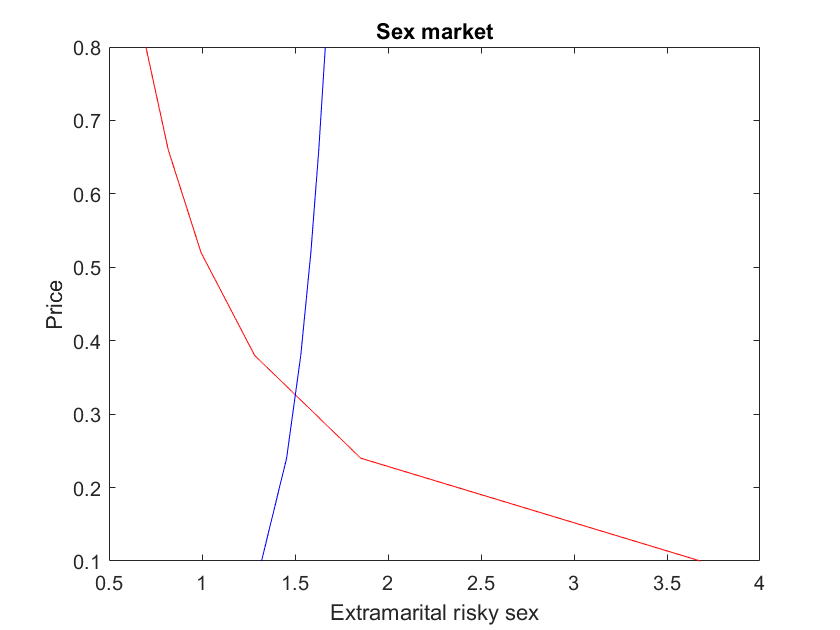
\includegraphics[angle=0,width=.5\textwidth]{figures/FIG14.png}   &
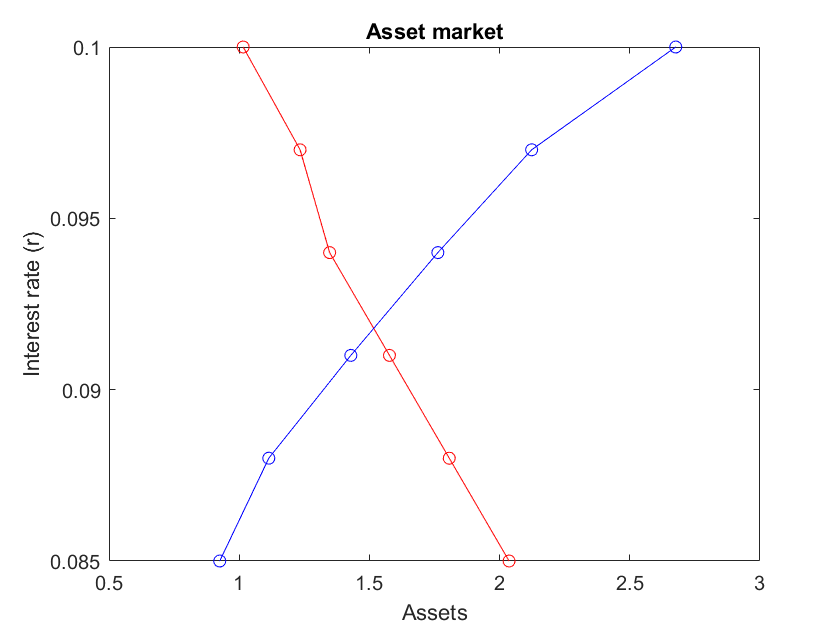
\includegraphics[angle=0,width=.5\textwidth]{figures/FIG15.png}
\end{tabular}
\end{center}
\label{fig:61}
\end{figure}

\begin{figure}[H]
\caption{Distributions}
\hspace{-2.0cm}
\begin{center}
\begin{tabular}{cc}
\multicolumn{1}{c}{(a) Asset Distribution} &
\multicolumn{1}{c}{(b) Income Distribution} \\
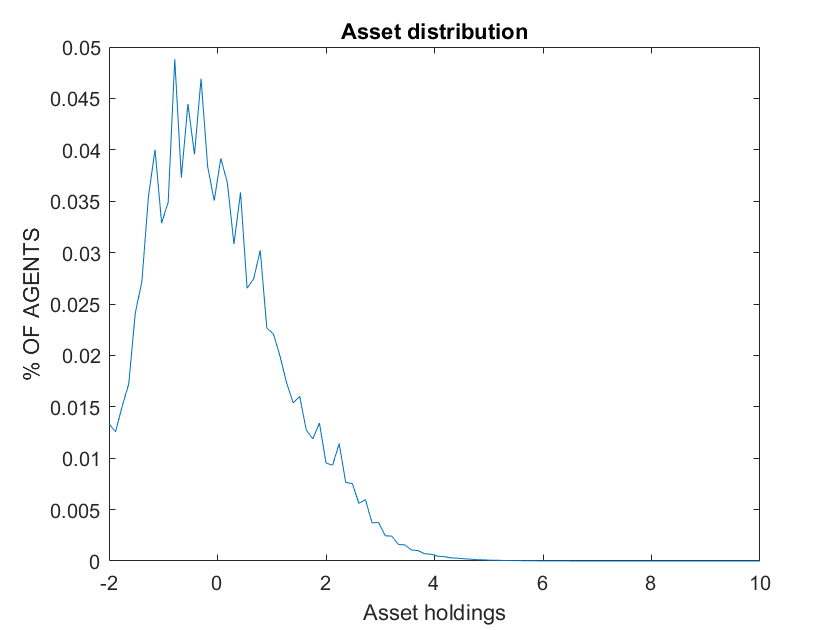
\includegraphics[angle=0,width=.5\textwidth]{figures/FIG9.png}   &
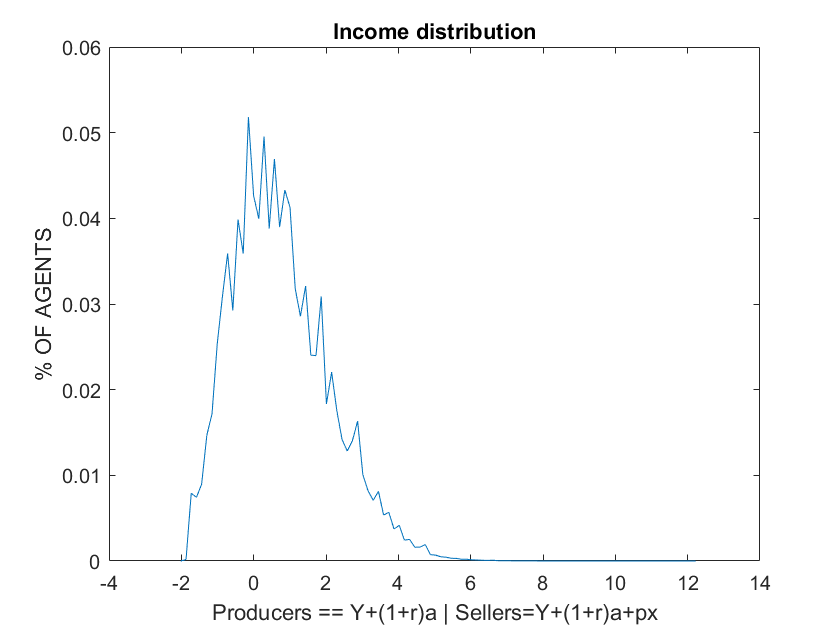
\includegraphics[angle=0,width=.5\textwidth]{figures/FIG10.png}
\end{tabular}
\end{center}
\label{fig:4}
\end{figure}


\subsection{Results Stage 1}
\begin{figure}[H]
\caption{Evolution of the prevalence overtime}
\hspace{-2.0cm}
\begin{center}
\begin{tabular}{c}
\multicolumn{1}{c}{Evolution of the prevalence overtime} \\
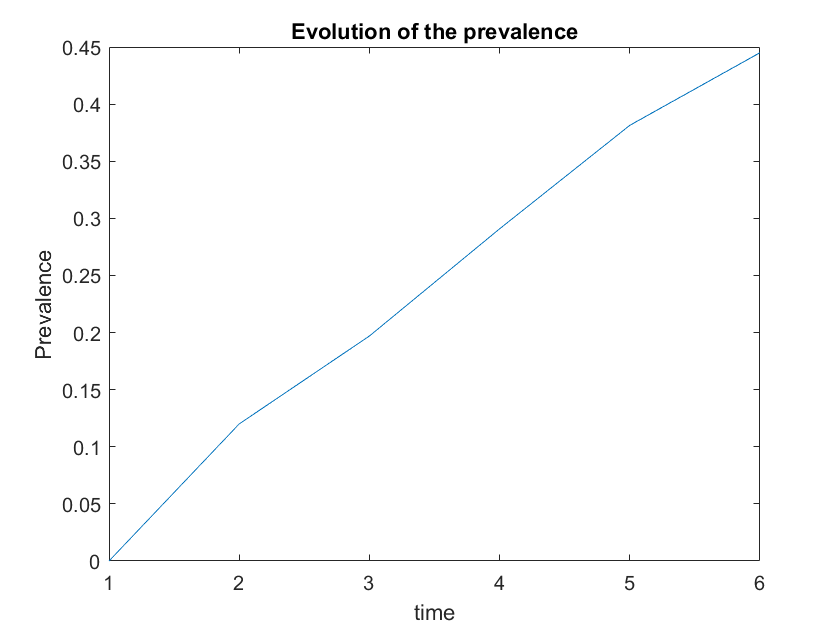
\includegraphics[angle=0,width=.5\textwidth]{figures/PREV.png}
\end{tabular}
\end{center}
\label{fig:6}
\end{figure}
\newpage

\section{Results}





\clearpage
